\begin{figure}[htbp]
  \centering
  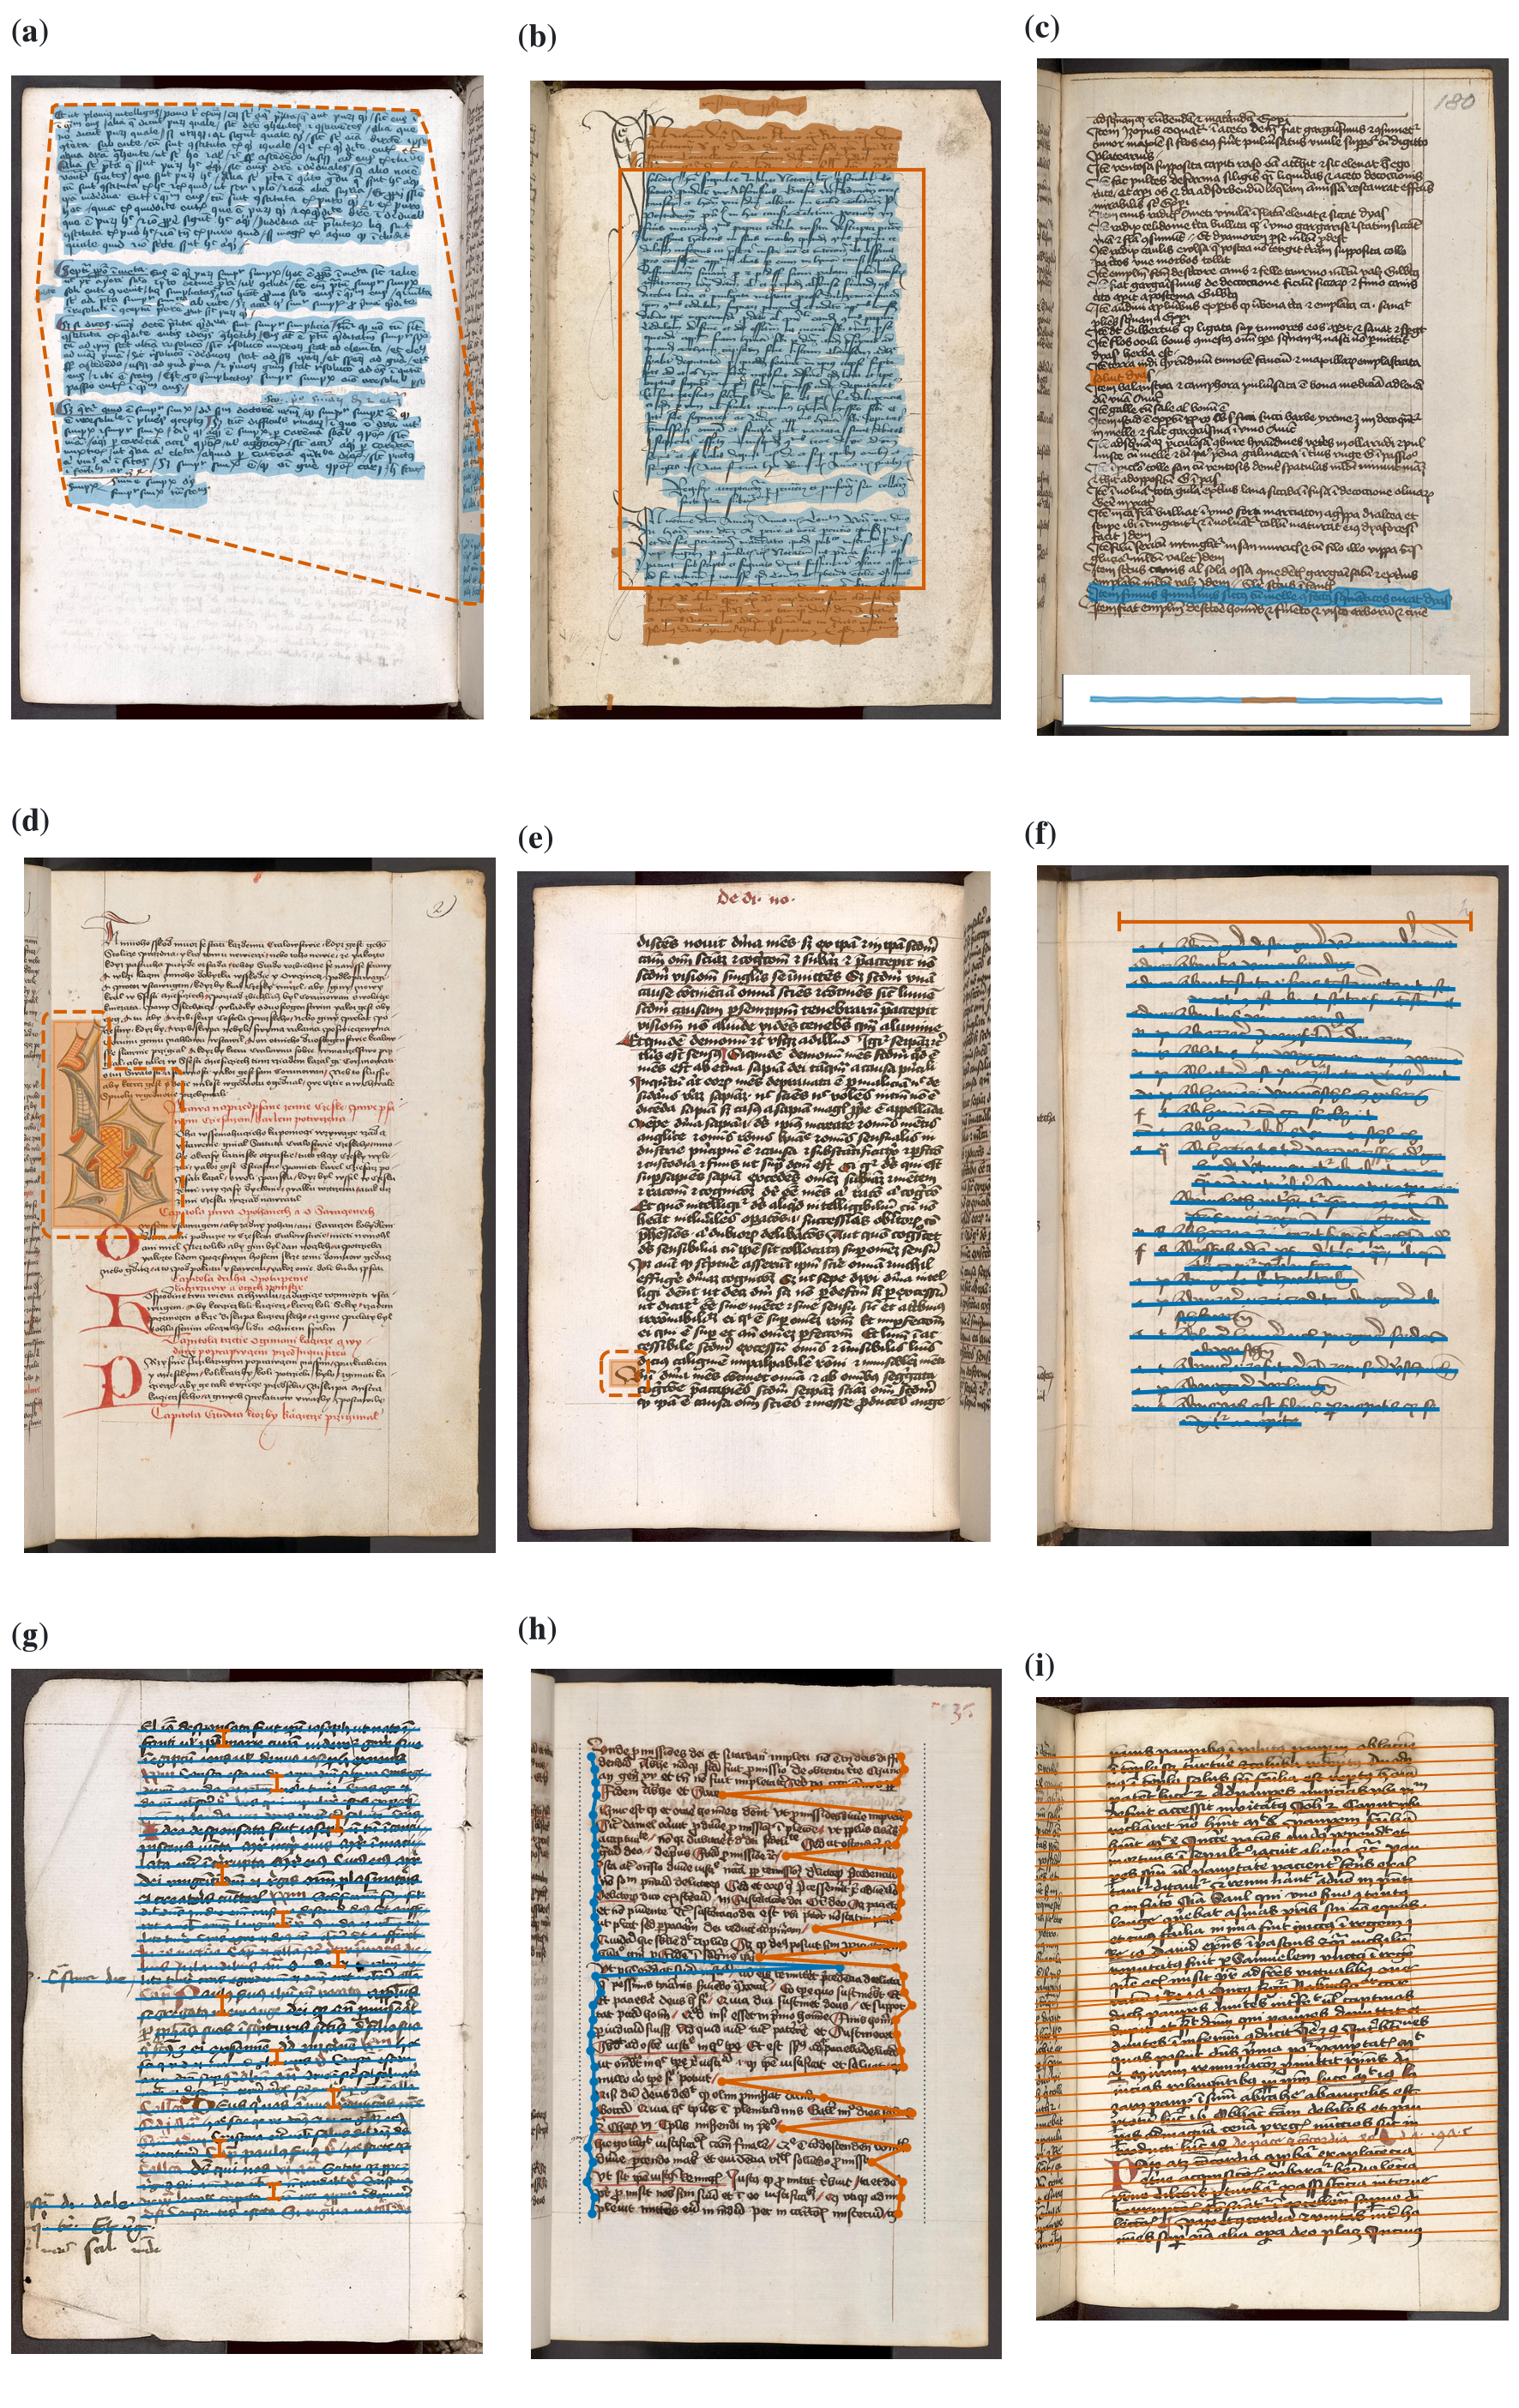
\includegraphics[width=15.00cm]{figures/geometry_features_on_page.png}
  \caption{The geometric features drawn on pages of the dataset: (a) the union of the line polygons (blue) and its convex hull (dashed), on ive19\_10v (\texttt{convexity} 0.693); (b) the written space (blue), the rectangle of its area and the folio's proportions centred on it, and the written space outside it (vermillion), on via6\_197r (\texttt{outside\_ratio} 0.205); (c) the longest and the shortest line measured, and below, their polygons centred on each other, on xie5\_180r (\texttt{dice\_median} 0.661); (d) the graphic zones, on xviic22\_44r (\texttt{graphic\_total\_area\_ratio} 0.067); (e) the drop capitals, on ive23\_150v (\texttt{drop\_capital\_num\_isolated\_instances} 1); (f) the baselines measured (blue) and their zones' widths, on xvie11\_2r (\texttt{var\_coef} 0.351); (g) the baselines and, for every third pair, the distance between them, on ih4\_3v (\texttt{max\_gap\_std} 0.042); (h) the lines' left (blue) and right (vermillion) ends, from line to line, on vc7\_35r (\texttt{std\_right} 0.165); (i) each baseline's direction, drawn across the folio, on vh3\_92r (\texttt{pairwise\_angle\_diff\_mean} 0.821). Page images provided by Manuscriptorium (CC BY-NC 4.0).}
  \label{fig:geometry_features_on_page}
\end{figure}
